% !TEX root=/home/tavant/these/manuscript/src/manuscript.tex




\chapter{Parametric study of the dielectric characteristics}
\label{ch-2}

We uses the PIC simulation code described in \cref{ch-1} in order to perform a parametric study over the two aspect of the dielectric walls: the secondary electron emission, and the modification of the electrostatic boundary condition.
We observe there impact on the electron cross-field mobility, and the electron temperature.
A large discrepancy is observed between the sheath model of \cref{sec-sheath} and the PIC simulation results.

\minitoc


% 
% Structure \string:
% 
% {\bf II. Parametric study of the dielectric} 30 pages
% \begin{zzz}
%   This chapter takes the 1rst paper which uses Vivien's results.
% 
%   2.1 Fully metallic wall (no SEE, grounded).
% 
%   2.2 Impact of Dielectric layer without SEE
% 
%   2.3 Impact of SEE with grounded wall
% 
%   2.4 SEE and dielectric in the same time
% 
%   2.5 Discrepancy between $\mean{\Te}$, $\sigma_{PIC}$ and $\sigma_{theo} = \sigma_0 + (1 - \sigma_0) \frac{2 T_e}{\epsilon_0}$
% \end{zzz}

As introduced in \Cref{ch-1}, the \ac{HET} behaviour is dependent of the axial electron transport toward the anode across the magnetic barrier.
Two main phenomena are proposed to enhance the electron mobility,
\begin{itemize}
  \item the azimuthal instability \ac{ECDI}
  \item the electron emission
\end{itemize}
In order to compare quantitatively the relative importance of the two phenomena, we propose to conduct a parametric study on the dielectric wall characteristics.

As highlighted, the \ac{ECDI} rises due to the $E \times B$ electron drift, but saturate thanks to the axial convection model.
Before investigating the time dependent behaviour of the system, we focus in this \Cref{ch-2} on the average values at steady state.
The first section describe the parameters of the simulation, 
while the second section highlight the main characteristics of the simulation result.


% !TEX root=/home/tavant/these/manuscript/src/manuscript.tex

\section{Presentation of the study}
  \label{sec-params}
  
  
  
  As introduced in \Cref{ch-1}, the \ac{HET} behavior depends strongly on the axial electron transport toward the anode across the magnetic barrier.
  Two main phenomena are proposed to enhance the electron mobility,
  \begin{itemize}
    \item plasma instabilities and in particular the azimuthal \ac{ECDI}, extensively studied in \cref{ch-5}
    \item the electron induced electron emission from the wall
  \end{itemize}
  In order to compare quantitatively the relative importance of the two phenomena, we propose to conduct a parametric study on the dielectric wall characteristics.
  As highlighted in the introduction and in \cref{ch-5}, the \ac{ECDI} rises due to the $E \times B$ electron drift, but saturates due to both the axial convection which limits the electron heating, and the ion-wave trapping.
  
  The first section describes the parameters of the simulation, 
  while the second section highlights the main characteristics of the base simulation results (electron mobility, plasma potential, electron mobility, etc.).
  The other sections of the chapter present the results of the parametric study on the wall characteristics\string: first we study in \cref{sec-diel_layer} the influence of the dielectric layer, then in \cref{sec-see} the secondary electron emission is analyze, and lastly we combine the two characteristics in \cref{sec-fulldiel}.

  The simulation domain corresponds to the exit plane of the thruster.
  Hence, a neutral pressure $P_n$ of 0.1~mTorr and a plasma density $n_e$ of $\sn{1}{17}$ m$^{-3}$ are used.
  The fixed axial electric field and radial magnetic field are $E_z=\sn{2}{4}\,\volt\per\meter$ and $B_r=200$ G, respectively.
  The rectangular \acs{2D} domain measures $L_r=2$~cm in the radial dimension and $L_{\theta}=0.5$~cm in the azimuthal direction.
  The axial length used for the convection is set to $L_z=1$~cm.
  It is important to note that the results shown in this chapter have been obtained at the beginning of my thesis, before the study of the convection presented in \cref{ch-1}.
  Hence, in this chapter we use the convection model of \citet{lafleur2016a}.
  However, we have validated that the convection model used does not modify the results under the conditions studied.
  The numerical parameters are chosen to respect the stability criterion of \ac{PIC} simulation, and are presented in \Cref{parameters}
  
  \begin{table}[htbp] %PIC parameters
       \centering
       \ra{1.3}
       \caption{\label{parameters} Standard operating and numerical parameters used in the 2D PIC simulations of an HET.  The simulation results are given as representative values.}
       \begin{tabular}{@{}r c c c@{}} 
          \toprule
          {\bf Physical Parameter} & notation & Value & Unit \\
          \midrule
          Gas & & Xenon & - \\
          Domain dimensions & $L_{x} \times L_{y} \times L_{z}$ & $2.0 \times 0.5 \times 1.0$ & [cm$^3$] \\
          Radial magnetic field & $B_{0}$                    & $200$                 & [{G}] \\
          Axial electric field & $E_{0}$                    & $2 \times 10^{4}$     & [{Vm}$^{-1}$] \\
          Mean plasma density & $n_{0}$                    & $3 \times 10^{17}$    & [{m}$^{-3}$] \\
          Initial electron temperature & $\Te_{,0}  $               & $10.0$                 & [{V}] \\
          Initial ion temperature & $T_{i,0}   $               & $0.1$                 & [{V}] \\
          Secondary electron temperature & $T_{see}   $               & $1.0$                 & [{V}] \\
          Neutral gas pressure & $P_{n}     $               & $1.0$                 & [{mTorr}] \\
          Neutral gas temperature & $T_{n}     $               & $300$                 & [{K}] \\
          Neutral gas density & $n_{g}     $               & $3.22 \times 10^{19}$ & [{m}$^{-3}$]\\
          \midrule
          {\bf Simulation Parameter} &  &   &  \\
          
          Time step & $\Delta t  $                      & $4 \times 10^{-12}$ & [{s}] \\
          Cell size & $\Delta x = \Delta y$ & $2 \times 10^{-5}$  & [{m}] \\
          Number of particles per cell & $N/NG      $                      & $80$                & [{part/cell}] \\
          \midrule
          {\bf Typical quantities} &  &  &  \\ 
          Electron plasma frequency & $\omega_{pe}$               & $3.1 \times 10^{10} $  & [rad/s]\\
          Ion plasma frequency & $\omega_{pi}$               & $36 \times 10^{6} $  & [rad/s]\\
          Electron cyclotron frequency & $\omega_{ce}$               &  $3.5\times 10^{9}$  & [rad/s] \\
          Electron Larmor radius & $r_{Le}$                    & 6$\times 10^{-4}$    & [m] \\
          \bottomrule
       \end{tabular}
    \end{table}
  
  
  The simulation is initialized with a uniform density of particles, following a Maxwellian distribution with temperatures $\Te_{,0}$ and $\Ti_{,0}$ for the electrons and the ions, respectively.
  
  
% !TEX root=/home/tavant/these/manuscript/src/manuscript.tex

\section{Canonical simulation results}
  \label{sec-canonical}
  
  The {\it canonical} case is the reference case that will be extensively described and commented.
  It will be used then to analyse and quantify the effects of the two aspect of the dielectric walls:
  \begin{itemize}
    \item the dielectric layer on the plasma potential, analysed in  % \cref{sec-dielectric_layer}
    \item the electron emission, analysed in %\cref{sec-see}
  \end{itemize}
  
  
  \Cref{fig-profiles} shows the radial profiles of the electron and ions densities averaged azimuthally.
  We can see the sheath close to the wall where the electron density fall rapidly compare to the ions.
  
  
  \begin{figure}[hbtp]
    \centering
    \includegraphics[width=\defaultwidth]{density_profile.pdf}
    \caption{Radial profile of the ion and electron densities at steady state.}
    \label{fig-profiles}
  \end{figure}
% !TEX root=/home/tavant/these/manuscript/src/manuscript.tex

\section{Modeling the dielectric layer }
  \label{sec-diel_layer}
  
  The first effect of the wall material studied is effect of adding a layer of dielectric material with its own permittivity, as introduced in \Cref{sec-diel}.
  The simulation parameters are the same as in the canonical case, presented in \cref{sec-canonical}, but the plasma is separated from the ground wall by a dielectric layer of 3~cm.
  Hence, the distance between the grounded electrodes is $2.6\,\milli\meter$.
  The relative permittivity of the dielectric is $\epsr=25$.
  %% SEE runs 250et 257 ?? Ly=1cm, Diel avec et sans SEE
  
  \Cref{fig-diel_radial_Er} shows the radial profile of the radial electric field $E_R$ at $t=10\,\micro\second$ averaged in the azimuthal direction.
  The plasma domain starts at $r=0$ and finishes at $r=2\,\centi\meter$.
  We note the jump in the value of the electric field at the plasma-wall transition.
  This jump is due to the surface charges.
  We can also notice that in the dielectric layer, in $r < 0$ and $r > 2\,\centi\meter$, the radial electric field is close to zero, compared to the value in the sheath.
  
  \begin{figure}[hbt]
    \centering
    \includegraphics[width=\defaultwidth]{diel_average_radial_electric_field}
    \caption{Radial profile of the radial electric field $E_R$ averaged in the azimuthal direction at $t=10\,\micro\second$. The plasma domain starts at $r=0$ and finishes at $r=2\,\centi\meter$. The dielectric length is $L_{\\rm Diel} = 3\,\milli\meter$.  }
    \label{fig-diel_radial_Er}
  \end{figure}
  
  The next sections investigate the impact of the dielectric layer on the plasma characteristics, and highlight the plasma-wall interaction.
  
  \subsection{Effect of the dielectric layer} \label{subsec-effect_mob}
    
  
  The simulation results are qualitatively the same as in the case without the dielectric layer.
  As an example, \Cref{fig-mod_diel_comp} shows the temporal evolution of the axial electron mobility with and without the dielectric layer.
  We see that the results for the electron temperature and mobility are similar.
  The low amplitude oscillation of the case with the dielectric decreases slightly slower.
  
  \begin{figure}[hbt]
    \centering
    \includegraphics[width=\defaultwidth]{Dielectric_noSEE_temporal.pdf}
    \caption{Temporal evolution of (left) the axial electron mobility and (right) the electron temperature with and without the dielectric layer modeled.}
    \label{fig-mod_diel_comp}
  \end{figure}

  
  \subsection{Near-wall and in-wall parameters} \label{subsec-nearwall}
    In this section, we focus on the surface charge and the near-wall electric field.
    \Cref{fig-sigma_time} shows the temporal evolution of the surface charge at one point of the wall.
    The position has been chosen to be the center ($L_{\theta} = 0.25$~cm) of the lower wall, but the observations are similar at other positions.
     
    \begin{figure}[hbt]
      \centering
      \includegraphics[width=\defaultwidth]{temporal_sigma}
      \caption{Temporal evolution of the surface charge $\sigma$ at one position of the lower dielectric wall}
      \label{fig-sigma_time}
    \end{figure}

    We can see on \cref{fig-sigma_time} that the value of the surface charge start by decreasing significantly (increasing in absolute value), due to the hot electrons that reach quickly the walls.
    Then, $\sigma$ growth and around a mean value close to $-3.5 \,\micro\coulomb/\square\meter$ and an amplitude of approximately $1.2 \,\micro\coulomb/\square\meter$.
    
    \cref{fig-indiel} shows the azimuthal evolution of the radial electric field inside the dielectric layer.
    The electric field is given at three different positions ($r=0.2, 0.9,$ and $1.8\,\milli\meter$ away from the plasma-wall interface) to highlight its evolution.
    We can see that, even thought there is no charge in the dielectric, the amplitude of the electric field decreases when going further away from the plasma.
    This is due to the \ac{2D} Poisson equation, which smooth-out the inhomogeneity.
     
    \begin{figure}[hbt]
      \centering
      \includegraphics[width=\defaultwidth]{Radial_electric_feld_in_diel.pdf}
      \caption{Azimuthal evolution of the radial electric field inside of the dielectric layer at three different positions; the reference $r=0$ is the plasma-wall interface, the grounded electrode is in $r=-3\,\milli\meter$.}
      \label{fig-indiel}
    \end{figure}

    
  \subsection{Dielectric model comparison} \label{subsec-modelcomp}
  
  \inlinenote{Anne: {\bf Beaucoup de remarques sur cette partie: pas assez claire, décrire plus les valeures observées, etc. Voir les notes sur le pdf (22 juillet)}}
  
  As introduced in \cref{sec-diel}, a simplified approach to model the effect of the surface charges on the plasma is to use a Neumann boundary condition \citep{taccogna2019}
  \begin{equation} \label{eq-neuman}
    E_r = \frac{\sigma}{\epsilon_0}.
  \end{equation}
  \Cref{eq-neuman} uses two approximations\string:
  \begin{itemize}
    \item one dimensional
    \item No electric field in the dielectric
  \end{itemize}
  We have already seen in \cref{fig-indiel} that the electric field in the dielectric is not zero, but instead it oscillates in respect to the azimuthal instability present in the plasma.  
  \Cref{fig-spacial_comparaison} shows the radial electric field at the wall and compares it to would be obtained by \cref{eq-neuman}.
  We can see that the two values are of the same order of magnitude, close to $-500$~kV/m.
  However, the two values are not equal, as they oscillates around their mean value.
  We can see that the surface charge oscillates more than the actual electric field obtained by solving the Poisson equation.

\begin{figure}[hbt]
  \centering
  \includegraphics[width=\defaultwidth]{Radila_electric_field.pdf}
  \caption{Azimuthal evolution of the radial electric field at the plasma-wall interface and the electric field that would be due to the surface charge using \cref{eq-neuman}.}
  \label{fig-spacial_comparaison}
\end{figure}
\renewcommand\subfigurewidth{0.45\textwidth}

  As a conclusion, we have observed that the dielectric layer does not change the simulation results much, but it can modify the surface processes.
  The model use here for the dielectric layer does not modify the performance of the simulation, while allowing to take into account the \ac{2D} effects.
  In this section, no secondary electron emission has been taken into account.
  In \cref{sec-fulldiel}, we will discuss the influence of using the simplified \cref{eq-neuman} in the case where secondary electron emission is important.

  
% !TEX root=/home/tavant/these/manuscript/src/manuscript.tex

\section{Effect of electron emission}
  \label{sec-see}
  
  In \Cref{sec-canonical}, the walls are not emissive.
  However, the dielectric ceramic used in \ac{HET} can emit electrons \citep{villemant2018,barral2003a}.
  The electron emission model used, introduced in \cref{sec-modelused}, has three parameters $\proba_0, \crover, \probamax$, such that the emission probability depends on the kinetic energy of the incident electron $\ek$ as
  \begin{equation} \label{eq-barral_second}
    \proba = \min \lp \proba_0 + (1 -  \proba_0) \frac{\ek}{\crover}, \probamax    \rp.
  \end{equation}
  
  The value of parameters are summarized in \cref{tab-tabe_parameters_see}.
  The crossover energy $\crover$ is varied from as low as 4~V, corresponding to a very emissive material, to as high as 200~V, a less emissive material.
  
  \begin{table}[hbtp]
  \ra{1.3}
    \centering
    \caption{Parameters of the electron emission probability model}
    \label{tab-tabe_parameters_see}
    \begin{tabular}{@{}ll@{}} \toprule
    Parameter & value  \\ \midrule
    $\proba_0$ & 0.5  \\
    $\probamax$ & 2.9 \\
    $\crover$   &  4  -- 200 V\\
    \bottomrule
    \end{tabular}
  \end{table}
  
  \begin{figure}[hbtp]
    \centering
    \includegraphics[width=\defaultwidth]{SEE_models}
    \caption{Illustration of the electron emission model of \cref{eq-barral_second} compared to a Maxwellian energy distribution function of temperature of 45~V, with $\crover=35.04$~V.}
    \label{fig-see_illustration}
  \end{figure}
  
  \Cref{fig-see_illustration} shows the electron emission probability for $\crover=35.04$~V compared to a Maxwellian \ac{EEDF} of temperature of 45~V.
  We can see that the saturation of $\proba$ at $\probamax$ happens only for the very high energy tail.
  In the simulation, we can only measure the average electron emission yield, also named emission rate, 
  \begin{equation} \label{eq-seeyield}
    \rate = \frac{\Gamma_{\rm emitted}}{\Gamma_{\rm incident}} = \frac{\iiint v_r \proba(\vect{v}) f(\vect{v}) d^3v}{\iiint v_r  f(\vect{v}) d^3v}.
  \end{equation}
  In general, \cref{eq-seeyield} cannot be calculated analytically.
  However, if we suppose that the \ac{EEDF} is Maxwellian and neglect the saturation at $\probamax$, \cref{eq-seeyield} yields
  \begin{equation} \label{eq-seemaxw}
    \ratemaxw(\Te) = \proba_0 + (1 - \proba_0) \frac{2 \Te}{\crover}.
  \end{equation}
  The saturation at $\probamax$ can be neglected as we have seen that it only affects a small part of the electron population, see \cref{fig-see_illustration}.
  \inlinenote{Add the exact calculation and the relative error ? \\Anne: oui. si trop long, a mettre en annexe.}
  
  \subsection{Impact of the electron emission of the mobility} \label{subsec-param-mob}
    
  The effects of the electron emission at the wall on the electron axial mobility are presented in \Cref{fig-mob-epsstar}.
  The measured mobility $\mobpic$ are shown, as well as the effective mobility $\mobeff$, the saturation estimate $\mobeffsat$ and the classical mobility $\mobcla$, defined in \cref{sec-transport} respectively by \cref{eq-mudef}, \cref{eq-defmobeff}, \cref{eq-mobeffsat} and \cref{eq-mobclas}.
  The values are averaged in time between $t=5 \mus$ and $t=10\mus$, and in space over the azimuthal and radial directions.
  \inlinenote{Anne: For epsilon=0, we have the values presented in section 2.2 without dielectrics.}
  \begin{figure}[hbtp]
    \centering
    \includegraphics[width=\defaultwidth]{parametric_mobs_eps_complete.pdf}
    \caption{Evolution of the electron mobility as a function of the crossover energy $\crover$. In blue $\mobpic$ is the mobility measured in the simulations, while $\mobcla, \mobeff$ and $\mobeffsat$ in purple, red and green respectively are calculated with \cref{eq-mudef,eq-mobclas,eq-defmobeff,eq-mobeffsat}. The three regimes {\bf I, II} and {\bf III}, described in \cref{subsec-regimes} are identified.}
    \label{fig-mob-epsstar}
  \end{figure}
  
  
  As expected, the classical mobility in  \cref{fig-mob-epsstar} is underestimated by more than one order of magnitude compared to $\mobpic$.
  The effective mobility $\mobeff$ and the effective mobility at saturation $\mobeffsat$  are much closer to $\mobpic$, with an underestimation of roughly 10\% and 30\% respectively.
  The mobility measured in the simulation does not evolve much with the electron emission, even for very high emission rate, i.e very low values of $\crover$.
  
  On the other hand, $\mobeffsat$ decreases slightly when $\crover$ decreases from around 40V to lower values.
  However, it still provides a reasonable approximation of the electron enhanced mobility, even with high electron emission rate. 
  
  \subsection{Near wall conductivity}
  
  The results presented in \cref{subsec-param-mob} are spatially averaged.
  However, the mobility coming from the  instability is expected to be higher where the instability is larger, hence at the center of the channel.
  On the other hand, the mobility due to wall emission is located close to the wall \citep{morozov1972}.
  
  \Cref{fig-radial-data} presents the radial profiles of the mobility measured in the \ac{PIC}  simulations without electron emission and for three values of $\crover$.
  On the left, the measured mobility $\mobpic$ is shown and on the right it is the effective mobility $\mobeff$ given by \cref{eq-defmobeff}.
  
  \begin{figure}[hbtp]
    \centering
    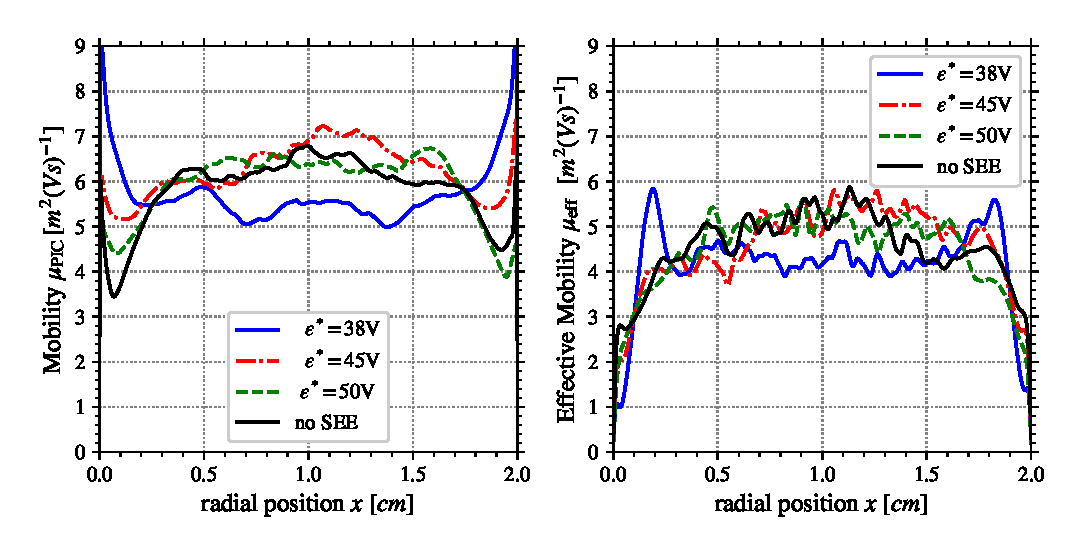
\includegraphics[width=\textwidth]{both_Mobility_SEE}
    \caption{Radial profile the electron mobility (left) measured in the \ac{PIC} simulations, and (right) given by \cref{eq-defmobeff}, for different wall emissivities. }
    \label{fig-radial-data}
  \end{figure}
  
  We can see in \cref{fig-radial-data} that the mobility measured $\mobpic$  in the center decreases by roughly 20\% as the emission rate increases.
  This observation is in agreement with $\mobeffsat$ observed in \cref{fig-radial-data,fig-mob-epsstar}.
  This is due the electron temperature $\Te$ which decreases from around $\Te=45$V at $\crover=200$V to $\Te=30$V at low $\crover$ (the evolution of $\Te$ can be seen in \cref{fig-Tevsproba}).
  
  On the other hand, the near wall mobility increases significantly on $\mobpic$ (almost by a factor of 2) with the increase of the electron emission.
  However, we do not see this evolution on $\mobeffsat$, meaning that it indeed comes from another physical mechanism than the \ac{ECDI}.
  
  
  \subsection{Three different regimes}
  \label{subsec-regimes}

  In \Cref{fig-mob-epsstar}, three regimes have been identified.
  Regime {\bf I} corresponds to low values of $\crover$ (lower than 35V), during which $\mobeffsat$ increases with $\crover$ but $\mobpic$ and $\mobeff$ decreases.
  Regime {\bf III} corresponds to high values of $\crover$ (higher than 50V), during which $\mobeffsat$, and  $\mobpic$ are roughlty constants, but $\mobeff$ increases slightly.
  Regime {\bf II} is a short transition regime, for $35 < \crover < 50$V.
  
  The different regimes are actually obvious when looking at the temporal evolution of the different variables.
  \Cref{fig-threeregimes}  presents the temporal evolution of the space average $\ratepic$ for three different
  values of $\crover$ , corresponding to three different regimes we have identified.
  In regimes {\bf I} and {\bf III}, $\ratepic$ reaches a steady state after a few microseconds.

  \begin{figure}[hbtp]
    \centering
    \includegraphics[width=\defaultwidth]{comparaison_3_regimes}
    \caption{Evolution as a function of time of the averaged electron emission rate $\ratepic$ in the three regimes observed (two stables, one with oscillations). The light green zones correspond to the periods when $\ratepic > \ratecr$}
    \label{fig-threeregimes}
  \end{figure}
  

  Regime {\bf I}, with low $\crover$, is characterized by a saturation of $\ratepic$ at a value between $\ratecr$ and 1, which leads to a non-monotonic potential profile.
  Regime {\bf III}, for higher $\crover$, is characterized by a steady state with a SEE rate lower than $\ratecr$.

  The transition between these two stable regimes (monotonic and non-monotonic sheath) passes by regime {\bf II}, an oscillating mode between the two stable regimes.
 As shown in \cref{fig-mob-epsstar}, regime {\bf II} is observed only in a narrow range of $\crover$.
 The oscillations of regime {\bf II} are shown in \cref{fig-threeregimes} up to $10\mus$ but have been observed for more than $40\mus$.
 Note that regimes {\bf I} and {\bf III} in \cref{fig-threeregimes} are obtained for $\crover = 38$~V and $\crover = 50$~V respectively, i.e. near the boundary of the unstable window (see \cref{fig-mob-epsstar}).
 Consequently, we observe a few oscillations before the steady-state is reached, as these cases are close to the bifurcation.
   
   
   The physical origin of the bifurcation can bee seen with the help of \cref{fig-dphivsTe}, which shows the evolution of the potential drop to the wall as a function of the electron temperature.
   It is computed using \cref{eq-seemaxw} for $\rate$ and \cref{eq-sheathhobbs} for the potential drop, which is summarized as 
   \begin{equation} \label{eq-dphi_vs_Te_Maxw}
     \begin{cases}
       \rate = \ratemaxw = \proba_0 + (1- \proba_0) \frac{2 \Te}{\crover} \\
       \dphi = \Te \ln \lp [1 - \rate] \sqrt{ \frac{m_i}{2 \pi m_e}}  \rp
     \end{cases}
   \end{equation}

   \begin{figure}[hbtp]
     \centering
     \includegraphics[width=\defaultwidth]{RSO_theo_sheath_bis}
     \caption{Plasma potential drop to the wall as a function of the electron temperature for different values of the cross-over energy $\crover$ using \cref{eq-dphi_vs_Te_Maxw}. The dashed line is $\dphi=\Te$. }
     \label{fig-dphivsTe}
   \end{figure}
   
   \Cref{fig-dphivsTe} shows the evolution of $\dphi$ as a function of $\Te$ obtained with \cref{eq-dphi_vs_Te_Maxw} using four different values of $\crover$. 
   We can see that, starting from low electron temperature, the potential drop increases with the electron temperature, resulting in a better screening of the electrons.
   This corresponds to regime {\bf III}.
   However, the $\dphi$ reaches a maximum, after which it drops sharply to zero and below.
   
   When the potential passes the maximum, the electrons are not screened by the sheath any more.
   Hence, the electrons reach the wall with a higher energy, resulting in a higher electron emission from the wall, hence a smaller potential drop.
   The sheath is unstable, and quickly attains a \ac{SCL} regime \citep{raitses2005}.
   
   In this regime, the sheath is not monotonic, and the model of \cref{eq-sheathhobbs} is no more valid, and the potential drop tends toward $\dphi \simeq \Te$ \citep{hobbs1967,goebel2008} \footnote{see \cref{sec-sheath} for more details}, shown in \cref{fig-dphivsTe}.
   This corresponds to regime {\bf I}.
   
   However, during regime {\bf I}, the electron power losses to the wall are very high, and they can exceed the gains.
   Hence, the electron temperature decreases.
   If $\Te$ decreases too much, the sheath can come back to the previous regime {\bf III}.
   The oscillations between regime {\bf I} and {\bf III} defines regimes {\bf II}.
      
   We have seen in \ref{fig-canon_Te_all} that without electron emission, $\Te$ is of the order of $45$~V.
   Using \cref{fig-dphivsTe}, we can expect to observe the transition between regime {\bf III} and {\bf II} for $\crover \gtrsim 60$~V, as for $\crover = 60$~V, the maximum of $\dphi$ is at $\Te\sim 25$~V, which is significantly lower than 45~V.
   
   The fact that regime {\bf II} appears at $\crover=50$~V could be explained because a smaller value of $\crover$ (hence a greater $\rate$) increases the electron losses, hence decreases the electron temperature at equilibrium.
   The evolution of the temperature with  $\rate$ is shown in \cref{fig-Tevsproba}.
   We can see that $\Te \simeq 45\,\volt$ for emission rate up to $\sigma = 0.8$, and decreases down to $\Te=30\,\volt$ for higher emission rates.
   Consequently, even if $\Te$ does indeed decreases when increasing $\crover$, it remains too large compared to the observations of \cref{fig-dphivsTe}.
   Hence, the cause of the difference if the threshold value for regime {\bf II} remain unknown for now.
   It will how be discussed again in \cref{ch-4}, using a modify plasma-wall interaction model.
   
   
  
% !TEX root=/home/tavant/these/manuscript/src/manuscript.tex

\section{Validation of the sheath model }
  \label{sec-sheath_validation}
  
  The \ac{PIC} simulations used here do not need any sheath theory in order to model the plasma-wall interaction.
  On the contrary, the rely on first principle models.
  Hence, they can be used in order to validate the sheath modeled introduced in \vref{sec-sheath} coming from the fluid theory.
  
  This sheath model of \vref{eq-sheathhobbs} links the plasma potential drop with the electron temperature on the electron emission rate.
  \Cref{eq-seemaxw} can be used to estimate the electron emission rate given the mean electron temperature measured in the simulations, corresponding statistically to the plasma bulk temperature.   
  In the \ac{PIC} simulations, \cref{eq-seeyield} can be computed by counting the number of electrons attaining the wall and emitted during a time-step.
  We note \ratepic this measurement.
  \vspace{1em}
   
  \begin{figure}[hbtp]
    \centering
    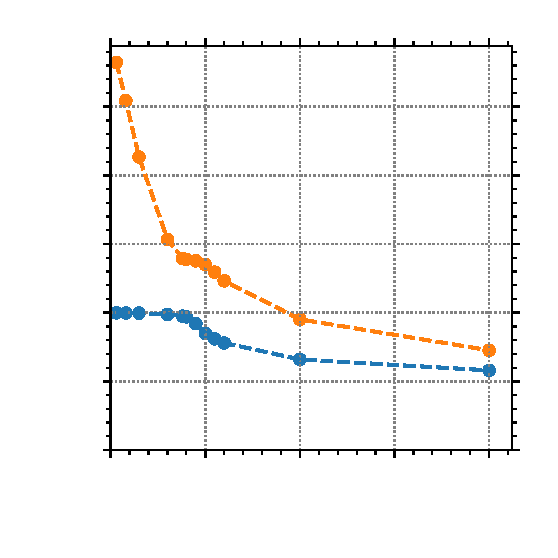
\includegraphics[width=\defaultwidth]{SEE_rates}
    \caption{Values of the electron emission rate $\ratepic$ (blue) measured in the simulation, and $ \ratemaxw$ obtained with \cref{eq-seemaxw} using the electron temperature showed in \cref{fig-Tevsproba}. }
    \label{fig-seeparamesMaxw}
  \end{figure}
  
  
  We can see in \Cref{fig-seeparamesMaxw} that the mean electron emission rate lies between 0.6 for large $\crover$ and 1 at low $\crover$.
  The saturation of \ratepic at 1 for high emissivity ( $\crover < 50 \volt$) was not expected from \ratemaxw.
  Indeed, \probamax is equal to 2.9, and the electron temperature in the bulk measured, when used in \cref{eq-seemaxw}, predicts a rate between 1.4 and 2.8.
  This discrepancy at low \crover is due to the \ac{SCL} regime.
  In \citet{hobbs1967}, the authors predict that in this regime, a potential well forms such that a fraction of the emitted electrons are returned to the wall, in order to maintain the effective emission rate to $\ratecr\sim1$.
  However, for $\crover > 50 \volt$, the sheath regime described in \vref{sec-sheath} should be valid.
   
  \begin{figure}[hbtp]
    \centering
    \begin{tabular}{cc}
      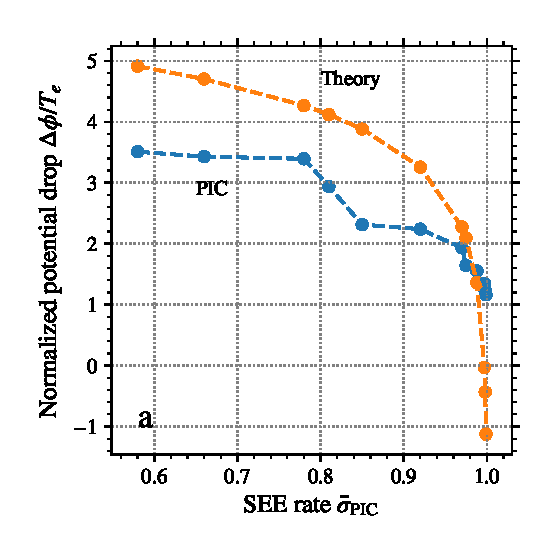
\includegraphics[width=3in]{phi_drop_6}
      &
      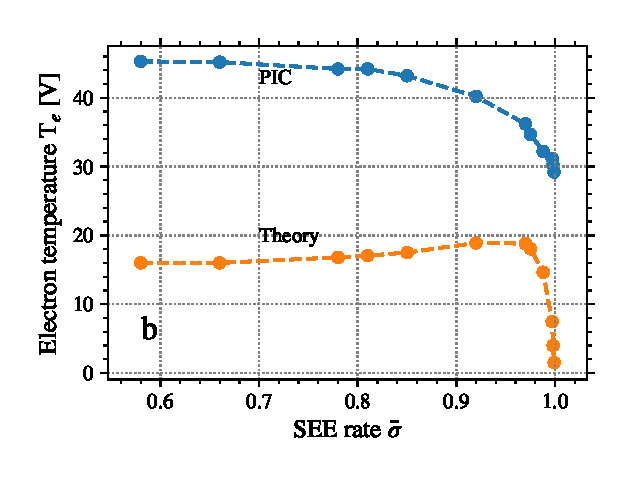
\includegraphics[width=3in]{Te_pic_2}
    \end{tabular}
    \caption{({\bf a}) Plasma potential drop to the wall normalized by the electron bulk as a function of the electron rate. {\bf $\Te$ is italic !}; ({\bf b}) Mean electron temperature measured in the \ac{PIC} simulations as a function of the electron emission rate \rate, measured as well in the simulations.  }
    \label{fig-Tevsproba}
  \end{figure}
  
  The electron temperature measured in the bulk of the simulation is presented in \cref{fig-Tevsproba}.{\bf b} for the same cases as in \cref{fig-seeparamesMaxw}.
  We can see that when \rate increases, $\Te$ monotonically decreases from 45V to around 30V.
  However, these values are not consistent with the measured emission rate \ratepic for $\crover > 50\volt$.

  \Cref{fig-Tevsproba}.{\bf a} shows the evolution of the potential drop to the wall measured in the \ac{PIC} simulation compared to the theory \vref{eq-total_drop} ({\bf OR is it \cref{eq-sheathhobbs} ...?}).
  As expected by \vref{eq-dphi_scl}, $\dphi$ measured in the simulation saturates to $\Te$ for high emission rate ($\ratepic \sim 1$).
  However, 
  We see that at low emission rate, the potential drop is significantly lower than expected.
  
  The sheath model of \cref{sec-sheath} used two hypotheses\string:
  \begin{itemize}
    \item Maxwellian electrons
    \item Isothermal evolution of the electrons
  \end{itemize}
  These two hypotheses will be confronted against the kinetic simulation in the next chapter.
  
  
   
% !TEX root=/home/tavant/these/manuscript/src/manuscript.tex

\section{Full dielectric model }
  \label{sec-fulldiel}
  
  We have observed the effects of the electron emission and the electrostatic boundary condition separately in \cref{sec-diel_layer,sec-see}, respectively.  
  In \Cref{sec-see}, we observed three regimes depending on the emission rate.
  At high emissivity, the sheath is space-charge limited, resulting in an inverse sheath.
  At low emissivity, we obtain the standard sheath model with electron emission.
  The transition between the regimes passes by a oscillating regime.
  
  In \Cref{sec-diel_layer} we observed that when there is no emission, the dielectric boundary condition for the potential does not change the simulation results.
  In this section, we investigate the interaction between the two characteristics of the dielectric walls, especially with a high emission rate.
  More precisely, regime {\bf II} is the most interesting, as it features a complex behavior.
  Hence, we use $\crover=45\,\volt$ to study the impact of the dielectric layer combined with the electron emission.
  
  The dielectric layer thickness is $L_{\rm Diel} = 3\,\milli\meter$, and the relative permittivity of the dielectric is $\epsilon_R=25$.
  The dimensions of the plasma domain is not modified between the case with and without the dielectric layer.
  Instead, it is the width between the grounded electrodes that is increased.
  
  \subsection{Impact of the dielectric boundary condition on the mobility with electron emission}
    
    \Cref{fig-temporal_mu} shows the temporal evolution of the electron mobility measured in the simulation $\mobpic$ for both cases, with and without the dielectric layer.
    We can see that the two variables are quite similar, with similar mean values and oscillation.
    Interestingly, the beginning of the simulations, up to $t=3\,\micro\second$, are almost identical.
    After this, the values are no more in phase, but follow a similar behavior.
    
    \begin{figure}[hbt]
      \centering
      \includegraphics[width=\defaultwidth]{dielectron_yesSEE_mobility}
      \caption{Temporal evolution of the axial electron mobility measured in the \acs{PIC} simulation with and without the dielectric layer between the plasma and the grounded electrodes. The crossover energy is $\crover=45\,\volt$, the length of the dielectric layer is $L_{\rm Diel}=3\milli\meter$ and its relative permittivity is $\epsilon_R = 25$.  }
      \label{fig-temporal_mu} 
    \end{figure}
    
    Hence, we conclude that results concerning the electron mobility obtained in \cref{sec-see} without the dielectric layer modeled will apply as well with the dielectric electrostatic boundary condition.
    In the next section, we analyze the plasma-wall interaction is more details.
    
  \subsection{Plasma-wall interaction}

  \begin{figure}[hbt]
    \centering
    \includegraphics[width=\defaultwidth]{dielectron_yesSEE_SEErate}
    \caption{Temporal evolution of the mean electron emission rate $\ratepic$ averaged over all the wall surface with and without the dielectric layer modeled, for the same value $\crover=45\,\volt$.}
    \label{fig-rso_diel}
  \end{figure}
  
  \Cref{fig-rso_diel} compares the temporal evolution of the mean electron emission rate $\ratepic$ for the same parameter $\crover=45\,\volt$, with and without the dielectric wall modeled.
  As previously, the dielectric width is $3\,\milli\meter$, and the electrodes are now $2.6\,\centi\meter$ apart (the geometry of the plasma domain is kept constant).
  As previously with the electron mobility, the two case present the same result at the beginning, up to $t=2\,\micro\second$.
  After that, the value of $\ratepic$ in the case with the dielectric layer oscillates lightly close to the critical value $\ratecr$, in contrast to the case without the dielectric layer that shows large variations.
  As \cref{fig-rso_diel} shows the values average over all of the wall, it can hide spatial variations.
  Hence the next figures present localized values.
  
  \Cref{fig-seediel_Er_time} shows the temporal evolution of the radial electric field in the sheath at the center of the azimuthal direction ($\theta=0.25 \,\centi\meter$) for {(\bf a)} the case with grounded wall, and {(\bf b)} the case with dielectric layers.
  Only the two millimeters close to the walls are shown, as the radial electric field in the plasma bulk is close to zero.
  On both cases, we can see the sharp transitions between the sheath with high electric field (low $\ratepic$) and the \ac{SCL} regime with low electric field, for which $\ratepic \simeq \ratecr$.
  Hence, in contrast to what could be understood from the mean \ac{SEE} rate in \cref{fig-rso_diel}, the case with dielectric layer do present the \ac{RSO} oscillations.
  For the case without the dielectric layers (\cref{fig-seediel_Er_time}.{\bf a}) the transitions between the left of the right wall are synchronous, as there appears simultaneously on the two walls.
  
  \begin{figure}[hbt]
    \centering
    \begin{tabular}{@{} c c}
      \subfigure{Er_2dcut_noDiel_RSO}{\Large a}{10,5} & 
      \subfigure{Er_2dcut_Diel_RSO}{\Large b}{10,5}
    \end{tabular}
    \caption{Temporal evolution of the radial electric field over 2$\,\milli\meter$ from the wall at the center of the azimuthal direction ($\theta=0.25 \,\centi\meter$) for {(\bf a)} the case with grounded wall, and {(\bf b)} the case with dielectric layers. }
    \label{fig-seediel_Er_time}
  \end{figure}

  On the other hand, the case with dielectric layers presents asynchronous transitions starting from $t=2\,\micro\second$ and later.
  This is why the \ac{RSO} oscillations could not be seen on $\ratepic$ in \cref{fig-rso_diel}.
  In addition, it seems that the left wall remains longer in the \ac{SCL} regime compared to the right wall.
  \Cref{fig-seediel_Er_time_theta} shows the temporal evolution of the radial electric field at the right wall and along the azimuthal direction for {(\bf a)} the case with grounded wall, and {(\bf b)} the case with dielectric layers.
  We see that for the case without the dielectric layer modeled, the sheath changes from the standard regime to the \ac{SCL} regime simultaneously along the radial direction.
  However, in the case with the dielectric layer, the sheath does not necessarily present the same regime at the same time along the azimuthal direction.
  This difference is due to the azimuthal electric field, that must be zero along the wall when the dielectric layer is not modeled, whereas it is not constrained with the dielectric layer modeled.
  
  \begin{figure}[!hbt]
    \centering
    \begin{tabular}{@{} c c}
      \subfigure{ch3_noDiel_2dcut_azimuthal}{\Large a}{10,5} & 
      \subfigure{ch3_Diel_2dcut_azimuthal}{\Large b}{10,5}
    \end{tabular}
    \caption{Temporal evolution of the radial electric field at the wall along the azimuthal direction for {(\bf a)} the case with grounded wall, and {(\bf b)} the case with dielectric layers. }
    \label{fig-seediel_Er_time_theta}
  \end{figure}
  
  
  To finish with, we show in \Cref{fig-surfacecharge} the temporal evolution of the electric field measured in the simulation at the wall and the electric field that corresponds to the surface charge $\frac{\sigma}{\epsilon_0}$ at the center of the azimuthal direction ($\theta=0.25 \,\centi\meter$).
  While the surface charge follows slightly the transitions between the \ac{SCL} and the usual sheath regime, it is significantly different from the measured electric field.
  Especially during the \ac{SCL} regime, where the surface charge shows large oscillations that is not observed on the radial electric field.
  
  \begin{figure}[!hbt]
    \centering
    \includegraphics[width=0.9\textwidth]{ch3_Er_vs_sigma_diel}
    \caption{Temporal evolution of (blue) the electric field at the wall and (orange) the electric field that corresponds to the surface charge $\frac{\sigma}{\epsilon_0}$ at the center of the azimuthal direction ($\theta=0.25 \,\centi\meter$) for ({\bf a}) the left wall and ({\bf b}) the right wall. The sign of the electric field is positive toward the wall.}
    \label{fig-surfacecharge}
  \end{figure}
  
  To summarized, we have compared in this section the results of the regime {\bf II} ($\crover=45\,\volt$) with and without the dielectric layer modeled.
  While the transitions between the \ac{SCL} (regime {\bf I} and the usual sheath (regime {\bf III}) is seen in both cases, when the dielectric layer is modeled the transitions are not synchronous between the two walls and along the azimuthal direction.
  Consequently, the sharp transitions of the averaged \ac{SEE} rate $\ratepic$ observed in regime {\bf II} without the dielectric layer is not observed.
  This could explain why this regime has not yet been observed experimentally, as it is very localized.
  Lastly, we observed that the surface charge does not presents the same evolution than the radial electric field at the wall, especially during the \ac{SCL} regime.
  This means that using the Neumann boundary condition to model the dielectric layer will certainly return different results.
  
  
% !TEX root=/home/tavant/these/manuscript/src/manuscript.tex

\section{Conclusion}
  \label{sec-conclusion_ch2}
  
